\documentclass{article}
\usepackage[slovene]{babel}
\usepackage{graphicx}
\usepackage{pgfplots}
\usepackage{float}
\usepackage{tabularx}
\usepackage{multirow}
\usepackage{booktabs}
\usepackage{array}
\pgfplotsset{compat=1.18}
\usepackage{amsmath}

\renewcommand{\figurename}{Slika}

\begin{document}

\title{Seminarska naloga pri predmetu Športna vzgoja}
\author{Urban Gajšek}
\date{\today}

\maketitle

\begin{center}
    \includegraphics[width=0.5\textwidth]{figures/univerza-v-ljubljani.png}
\end{center}

\newpage
\tableofcontents
\newpage

\section{Uvod in namen seminarske naloge}
Dandanes se ljudje premalo gibamo, še posebej tisti, ki imamo sedeče delo. Pomembno je, da smo redno fizično aktivni, saj s tem ohranjamo svoje zdravje in dobro počutje.
\paragraph{}
Namen seminarske naloge je ustvarjanje delovnega zvezka, s katerim bom dokazal, da znam uporabiti pridobljeno teoretično in praktično znanje za uresničevanje zastavljenih ciljev.

\section{Cilji, hipoteze, sredstva}
\subsection{Cilji}
\subsubsection{Cilji v moči}
Kot cilj sem si zadal, da bom v 30 dneh lahko izboljšal število opravljenih zgibov iz 15 na 20. Ta cilj sem si izbral, ker je zame dosegljiv in hkrati izziv, pa tudi zato, ker je zgib zelo koristna vaja za krepitev zgornjega dela telesa, katerega uporabljam pri svojem športu - veslanju na divjih vodah.
\paragraph{Mesečni plan:}
Pripravil sem si mesečni plan, za katerega menim, da mi bo omogočil doseči zastavljeni cilj, hkrati pa ne bo preveč obremenjujoč:

\begin{figure}[H]
    \centering
    \includegraphics[width=1\textwidth]{figures/Stange-mesecni-plan.png}
    \caption{Posnetek zaslona mesečnega plana za izboljšanje števila opravljenih zgibov v istem poskusu iz aplikacije Google Calendar.} 
    \label{fig:mesecni-plan}
\end{figure}

Plan je sledeč: Trikrat tedensko bom izvajal treninge na "štangah" oz. fitnesu na prostem, kjer bom izvajal vaje za krepitev zgornjega dela telesa - to bojo večinoma prav zgibi ali pa različne variacije zgibov. Če mi bo vspelo po vsakih dveh treninhig izboljšati število zgibov za vsaj 1, bom v trinajstih zastavljenih treningih dosegel svoj cilj.

\begin{center}
  \textbf{\Large Tedenski plan vadbe}
\end{center}

\vspace{0.5cm}

\begin{tabularx}{\textwidth}{|p{2.3cm}|p{0.5cm}|p{0.5cm}|p{2.3cm}|p{0.5cm}|p{2.3cm}|X|}
  \hline
  Pon & Tor & Sre & Čet & Pet & Sob & Ned \\
  \hline
  Štange Študentski domovi rožna dolina &  &  & Štange Študentski domovi rožna dolina & & Štange pri železniški postaji Nova Gorica & \\
  \hline
\end{tabularx}

\subsubsection{Cilji v prehrani}
Ker je prehrana zelo pomembna pri športni aktivnosti in pri regeneraciji in rasti mišič, sem si zadal tudi cilj, da bom v teh 30 dneh poskušal vsak dan zaužiti vsaj $130g$ beljakovin.

\subsection{Hipoteze}

Menim, da bom cilj dosegel prej kot v 30 dneh, saj že prej opazil, da lahko hitro napredujem pri zgibih, če redno treniram. Višjega cilja si nisem postavil, saj se velikokrat zgodi, da se kaj zalomi, in zmanjka časa za trening.
\paragraph{}
Menim tudi, da bo napredek sprva hiter, nato pa vse počasnejši, saj je to značilno za večino športnih aktivnosti.

\subsection{Sredstva}

\subsubsection{Analiza treningov}
Vask trening bom opravljal z športno uro (Xiaomi Mi Band 5), ki mi bo merila srčni utrip in na podlagi tega bo ocenila, koliko kalorij sem porabil.

\subsubsection{Dnevnik prehrane}
Prvi teden bom beležil tudi kaj sem pojedel, da bom lahko spremljal, če imam zadosten vnos beljakovin, pa tudi koliko kalorij sem zaužil.

\subsubsection{Preverjanje napredka}
Vsak trening bom zabeležil maksimalno število zgibov, ki jih bom opravil v enem poskusu. Da bodo testi med seboj čim bolj podobni, jih bom vedno opravljal tik po ogravnju in opravil toliko zgibov, kolikor bom zmogel. Število zgibov bom beležil v zvezku, na koncu pa bom podatke predstavil v obliki grafa.

\section{Izračun bazalnega metabolizma}
Bazalni metabolizem sem izračunal po Mifflin-St Jeorjevi formuli, ki izgleda takole:
\[
BMR = 10 * weight + 6.25 * height - 5 * age + 5 
\]

kjer je $BMR$ bazni metabolizem (v $kcal$), $weight$ teža v kilogramih, $height$ višina v centimetrih, $age$ pa starost v letih. Po izračunu sem dobil vrednost $1900 kcal$. Ta podatek bom uporabil pri računanju celotne porabe kalorij v dnevu. 

\section{Rezultati in razlaga}

\textbf{\Large Dnevnik prehrane in vadbe}

\vspace{0.5cm}

\begin{tabularx}{\textwidth}{|c|c|c|c|X|}
  \hline
  & \textbf{Obrok} & \textbf{Vnos kalorij} & \textbf{Vrsta in čas vadbe} & \textbf{Poraba kalorij} \\
  \hline
  \multirow{4}{*}{\textbf{Pon}} & Zajtrk & 442 & Trening na štangah & 2340 \\
                                & Kosilo & 611 & ob 8:40 & \\
                                & Večerja & 613 & & \\
                                & Malica/e & 357 & & \\
  \hline
  \multirow{4}{*}{\textbf{Tor}} & Zajtrk & 439 & Fitness Push workout & 2411 \\
                                & Kosilo & 882 & ob 17:00 & \\
                                & Večerja & 614 & & \\
                                & Malica/e & 192 & & \\
  \hline
  \multirow{4}{*}{\textbf{Sre}} & Zajtrk & 554 & Odbojka & 2194 \\
                                & Kosilo & 736 & ob 18:00 & \\
                                & Večerja & 658 & & \\
                                & Malica/e & 882 & & \\
  \hline
  \multirow{4}{*}{\textbf{Čet}} & Zajtrk & 430 & Trening na štangah & 2243 \\
                                & Kosilo & 891 & ob 15:05 & \\
                                & Večerja & 610 & & \\
                                & Malica/e & 199 & & \\
  \hline
  \multirow{4}{*}{\textbf{Pet}} & Zajtrk & 452 & / & 2099 \\
                                & Kosilo & 635 & & \\
                                & Večerja & 614 & & \\
                                & Malica/e & 248 & & \\
  \hline
  \multirow{4}{*}{\textbf{Sob}} & Zajtrk & 451 & Trening na štangah & 2466 \\
                                & Kosilo & 947 & ob 9:00 & \\
                                & Večerja & 377 & & \\
                                & Malica/e & 0 & & \\
  \hline
  \multirow{4}{*}{\textbf{Ned}} & Zajtrk & 555 & Tek v Panovcu & 2401 \\
                                & Kosilo & 625 & ob 10:00 & \\
                                & Večerja & 409 & & \\
                                & Malica/e & 88 & & \\
  \hline                                     
\end{tabularx}

Na dnevniku prehrane in vadbe je razvidno, da sem se treningov držal po planu, glede vnosa beljakovin pa sem sicer v povprečju zaužil $142g$ na dan, ampak sem jih v petek zauil le $117g$. Na splošno sem zadovoljen z rezultati v zvezi s sledenjem plana.

Na spodnjem grafu je razvidno, kako se je spreminjalo število zgibov, ki sem jih opravil v enem poskusu, skozi 13 treningov.

\begin{figure}[H]
\centering
    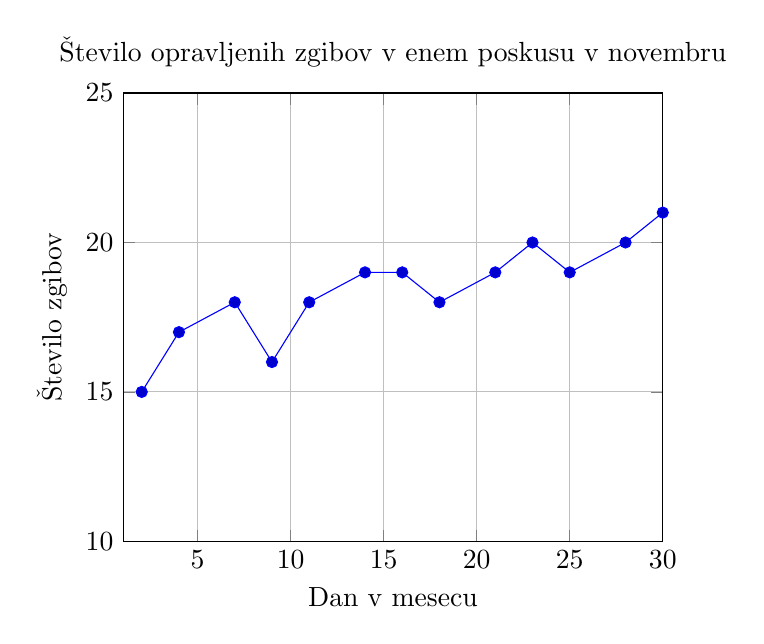
\begin{tikzpicture}
      \begin{axis}[
          title={Število opravljenih zgibov v enem poskusu v novembru},
          xlabel={Dan v mesecu},
          ylabel={Število zgibov},
          grid=major,
          xmin=1, xmax=30,
          ymin=10, ymax=25
        ]
        \addplot coordinates {
          (2,15) (4,17) (7,18) (9,16) (11,18) (14,19) (16,19) 
          (18,18) (21,19) (23,20) (25,19) (28,20) (30,21)
        };
      \end{axis}
    \end{tikzpicture}
\caption{Napredek pri številu zgibov v enem poskusu skozi 13 treningov.}
\end{figure}

\paragraph{}
Iz grafa je razvidno, da je število opravljenih zgibov v enem poskusu naraščalo skoraj linearno, z manjšimi odstopanji, 20 zgibov pa sem dosegel že 10. trening.

\begin{figure}[H]
    \centering
    \includegraphics[width=0.4\textwidth]{figures/srcni-utrip.jpg}
    \caption{Posnetek zaslona aplikacije Mi Fit, ki prikazuje srčni utrip med treningom.} 
    \label{fig:srcni-utrip}
\end{figure}

\paragraph{}
Posnetek zaslona aplikacije Mi Fitness, ki prikazuje srčni utrip med treningom, je prikazan na sliki \ref{fig:srcni-utrip}. Povprečni uprip med treningom je bil $96bpm$, največji pa $122bpm$. Aplikacija je na podlagi srčnega utripa večji del treninga klasificirala kot "Light intensity". Rezultati so pričakovani, saj je bil trening sestavljen iz več serij zgibov, ki so bile med seboj ločene z dolgimi odmori, poleg tega pa glavna omejitev pri zgibih ni vzdržljivost, temveč moč. 

\paragraph{}
Slika \ref{fig:poraba-kalorij} pa prikazuje posnetek zaslona iz aplikacije Mi Fitness, iz katere je razvidno, da sem med treningom, ki je trajal $40 min$ porabil $215 kcal$. Glede na nizko aerobno intenzivnost treninga ter precej kratko trajanje, je poraba kalorij pričakovano nizka. Vredno pa je omeniti, da se pri treningih za moč porabi nekaj več kalorij še potem, ko se trening konča, saj telo potrebuje energijo za regeneracijo mišic.

\begin{figure}[H]
    \centering
    \includegraphics[width=0.4\textwidth]{figures/poraba-kalorij.jpg}
    \caption{Poraba kalorij med treningom, ter ostali podatki} 
    \label{fig:poraba-kalorij}
\end{figure}

\section{Zaključek in sklepi}

Plan prehrane in vadbe vsekakor ni bil optimalen, bil pa je zadosten, saj sem cilj seveda dosegel in celo presegel. Z rezultati sem zadovoljen. Ugotovil sem tudi, da trening na štangah pravzaprav ne porabi prav veliko kalorij, saj je povprečna intenzivnost nizka, pulz pa se dvigne le, ko dejansko opravljamo zgibe, med pavzo pa precej pade. 

\section{Literatura in viri}

\begin{itemize}
  \item \textit{Mifflin-St Jeorjeva formula za izračun bazalnega metabolizma}: \\
  \texttt{https://nutrium.com/blog/mifflin-st-jeor-for-nutrition-professionals}

  \item \textit{Mi Fit aplikacija}: \\
  \texttt{https://play.google.com/store/apps/details?id=com.xiaomi.wearable}

  \item \textit{Google Calendar}: \\
  \texttt{https://calendar.google.com/calendar}

  \item \textit{My Fitness Pal}: \\
  \texttt{https://www.myfitnesspal.com/}

  \item \textit{Postavitev tabele - dnevnik prehrane in vadve}: \\
  \texttt{Smernice za izdelavo seminarske.docx}
\end{itemize}

\end{document}